\begin{figure}[t!]
    \begin{subfigure}[b]{0.5\textwidth}
    \centering
    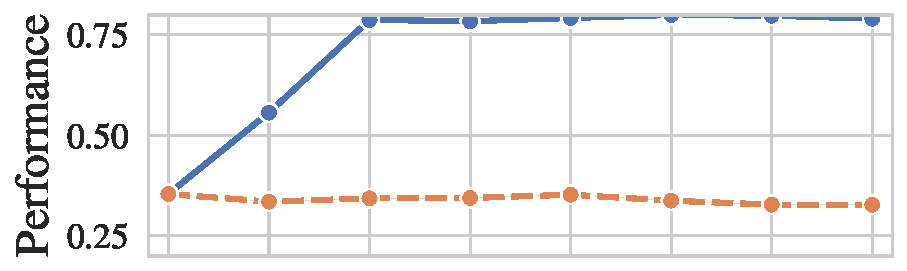
\includegraphics[width=0.8\columnwidth]{figures/fig_files/sft_evalmnli_matched-trainmnli_tight.pdf}
        \caption{MNLI Matched}
        \label{fig:subfig:improve}
    \end{subfigure}%
    \\
    \begin{subfigure}[b]{0.5\textwidth}
        \centering
    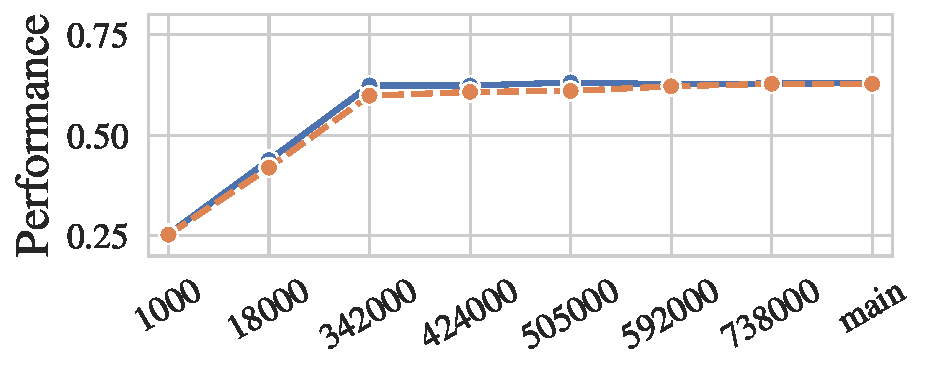
\includegraphics[width=0.8\columnwidth]{figures/fig_files/it_evalhellaswag_tight.pdf}
        \caption{Hellaswag}
        \label{fig:subfig:notimprove}
    \end{subfigure}
    \caption{Example of few-shot performance on different pre-training steps of the models that benefited (\ref{fig:subfig:improve}) and did not benefit from fine-tuning (\ref{fig:subfig:notimprove}). The \textcolor{snsblue}{\textbf{solid blue}} line represents the fine-tuned checkpoint, and the \textcolor{snsorange}{\textbf{dashed orange}} line represents the base checkpoint. The results of all datasets can be found in Figure~\ref{fig:sft-ckpt-perf} and Figure~\ref{fig:it-ckpt-perf}.}
    \label{fig:improve-and-notimprove-example}
\end{figure}